%==============================================================================
%== template for LATEX poster =================================================
%==============================================================================
%
%--A0 beamer slide-------------------------------------------------------------
\documentclass[5pt, final]{beamer}
\usepackage[orientation=portrait, size=a0,
            scale=1.25         % font scale factor
           ]{beamerposter}
           
\geometry{
  hmargin=2.5cm, % little modification of margins
}

%
\usepackage[utf8]{inputenc}

\linespread{1.05}
%
%==The poster style============================================================
\usetheme{sharelatex}

%==Title, date and authors of the poster=======================================
\title
[Agile Vorgehensmodelle, Master, WS 202425] % Conference
{ % Poster title
	Die Rolle des Scrum Masters: Moderation, Konfliktlösung und Teamförderung
}

\author{ % Authors
	Nico Riedlinger\inst{1}, Marc Weiss\inst{1}
}
\institute
[Very Large University] % General University
{
	\inst{1} HTWG Konstanz
}
\date{\today}



\begin{document}
	\begin{frame}[t]
		%==============================================================================
		\begin{multicols}{3}
			%==============================================================================
			%==The poster content==========================================================
			%==============================================================================
			
			\section{Introduction}
			
			In Ref.~\cite{ref1}...
			In Refs.~\cite{ref1,ref2}...
			On webpage~\cite{web}...
			
			
			\section{Result and discussions}
			
			\vskip1ex
			\begin{table}
				\centering
				\caption{This is a table with scientific results.}
				\begin{tabular}{ccccc}
					\hline\hline
					1 & 2 & 3 & 4 & 5\\
					\hline
					aaa & bbb & ccc & ddd & eee\\
					aaaa & bbbb & cccc & dddd & eeee\\
					aaaaa & bbbbb & ccccc & ddddd & eeeee\\
					aaaaaa & bbbbbb & cccccc & dddddd & eeeeee\\
					1.000 & 2.000 & 3.000 & 4.000 & 5.000\\
					\hline\hline
				\end{tabular}
			\end{table}
			\vskip2ex
			
			\subsection{SubSection}
			
			\vskip1ex
			\begin{figure}
				\centering
				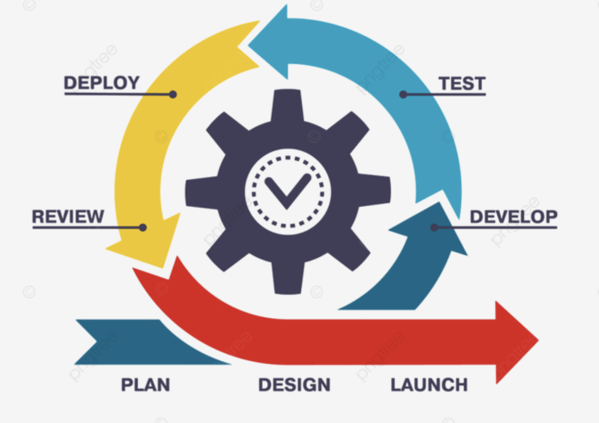
\includegraphics[width=0.95\columnwidth]{demo.png}
				\caption{This is a picture with scientific results.}
			\end{figure}
			\vskip2ex
			
			\subsection{SubSection, a very very very very very very long title}
			
			%==============================================================================
			%==End of content==============================================================
			%==============================================================================
			
			%--References------------------------------------------------------------------
			
			\subsection{References}
						
			\begin{thebibliography}{99}
				
				\bibitem{ref1} J.~Doe, Article name, \textit{Phys. Rev. Lett.}
				
				\bibitem{ref2} J.~Doe, J.~Smith, Other article name, \textit{Phys. Rev. Lett.}
				
				\bibitem{web} \url{http://www.google.pl}
				
			\end{thebibliography}
			%--End of references-----------------------------------------------------------
			
		\end{multicols}
		
		%==============================================================================
	\end{frame}
\end{document}
